\begin{figure*}
	\centering
	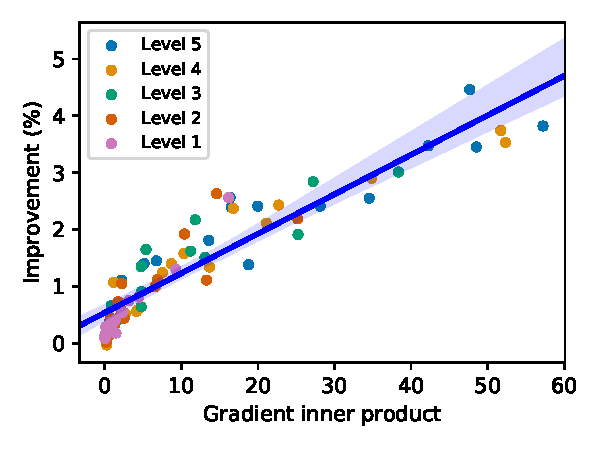
\includegraphics[width=0.48\textwidth]{plots/C10C_layer2_slow_gn_expand_final_grad_corr.pdf}
	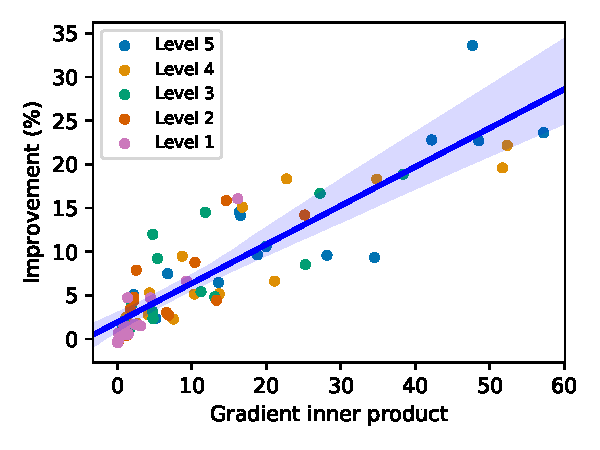
\includegraphics[width=0.48\textwidth]{plots/C10C_layer2_online_gn_expand_final_grad_corr.pdf}
	\caption{
		Scatter plot of the inner product between the gradients (on the shared feature extractor $\vtheta_e$) of
		the main task $l_m$ and the self-supervised task $l_e$, and the improvement in test error (\%) from Test-Time Training, 
		for the standard (left) and online (right) version. 
		Each point is the average over a test set, and each scatter plot has 75 test sets, from all 15 types of corruptions over five levels as described in \autoref{results_cc}.
		The blue lines and bands are the best linear fits and the 99\% confidence intervals.
		The linear correlation coefficients are $0.93$ and $0.89$ respectively, indicating strong positive correlation between the two quantities, as suggested by \Cref{main_theorem}.
	}
	\label{gradient_improve}
\end{figure*}

\section{Theoretical Results}
\label{theory}
This section contains our preliminary study of when and why Test-Time Training is expected to work.
For convex models, we prove that positive gradient correlation between the loss functions leads to better performance on the main task after Test-Time Training.
Equipped with this insight, we then empirically
demonstrate that gradient correlation governs the success of Test-Time Training on the deep learning model discussed in \Cref{results}.

Before stating our main theoretical result, we first illustrate the general intuition with a toy model.
Consider a regression problem where $x\in\R^d$ denotes the input,  $y_1\in\R$ denotes the label, and the objective is the square loss
$(\hat{y}-y_1)^2/2$ for a prediction $\hat{y}$.  
Consider a two layer linear network parametrized by $\mA\in\R^{h\times d}$ and $\vv \in\R^h$ (where $h$
stands for the hidden dimension).  
The prediction according to this model
is $\hat{y}=\vv^\top \mA x$, and the main task loss is
\begin{equation}
    l_m(x, y_1; \mA, \vv) = \frac{1}{2}\left(y_1 - \vv^ \top \mA x\right)^2.
\end{equation}
In addition, consider a self-supervised regression task that also uses the square loss and automatically generates a label $y_s$ for $x$. 
Let the self-supervised head be parametrized by $\vw\in\R^h$.  Then the self-supervised task loss is
\begin{equation}
    l_s(x, y_2; \mA, \vw) = \frac{1}{2}\left(y_2 - \vw^\top\mA x\right)^2.
\end{equation}
Now we apply Test-Time Training to update the shared feature extractor $\mA$ by
one step of gradient descent on $l_s$, which we can compute with $y_2$ known.
This gives us
\begin{equation}
    \mA' \leftarrow \mA - \eta\left( y_2-\vw^\top\mA x \right) \left(-\vw x^\top\right),
\end{equation}
where $\mA'$ is the updated matrix and $\eta$ is the learning rate.
If we set $\eta = \eta^*$ where
\begin{equation}
\label{magic_lr}
\eta^* = \frac{y_1 - \vv^\top \mA x}{\left( y_2 - \vw^\top \mA x \right)
	\vv^\top \vw x^\top x},
\end{equation}
then with some simple algebra, it is easy to see that the main task loss 
$l_m(x, y_1; \mA', \vv) = 0$.  
Concretely, Test-Time Training drives the main task loss down to zero with a single gradient step for a carefully chosen learning rate. 
In practice, this learning rate is unknown since it depends on the unknown $y_1$.
However, since our model is convex, as long as $\eta\opt$ is positive, it suffices to set $\eta$ to be a small positive constant (see details in the appendix).
If $x \neq 0$, one sufficient condition for $\eta^*$ to be positive (when neither loss is zero) is to have
\begin{align}
\label{equal_sign}
    \sign\left( y_1 - \vv^\top \mA x \right) = \sign\left( y_2 - \vw^\top \mA x \right)\\
    \text{and}\quad
    \vv^\top \vw > 0 \;.
\end{align}
For our toy model, both parts of the condition above have an intuition interpretation.
The first part says that the mistakes should be correlated, in the sense
that predictions from both tasks are mistaken in the same direction. The second
part, $v^\top \vw > 0$, says that the decision boundaries on the feature
space should be correlated. In fact, these two parts hold iff.
$\langle \grad l_m(\mA), \grad l_s(\mA)\rangle > 0$ 
(see a simple proof of this fact in the appendix). To summarize, if the gradients have
positive correlation, Test-Time Training is guaranteed to reduce the main task loss.
Our main theoretical result extends this to general smooth and convex loss functions.

\newpage
{\theorem	\label{main_theorem}
Let $l_m(x, y; \vtheta)$ denote the main task loss on test instance $x, y$ with
parameters $\vtheta$, and $l_s(x; \vtheta)$ the self-supervised task loss that only depends on $x$.
Assume that for all $x, y$,
$l_m(x, y; \vtheta)$ is differentiable, convex and $\beta$-smooth
in $\vtheta$,
and both
$\norm{\grad l_m(x, y; \vtheta)}, \norm{\grad l_s(x, \vtheta)} \leq G$ 
for all $\vtheta$.
With a fixed learning rate $\eta = \frac{\eps}{\beta G^2}$, 
for every $x, y$ such that 
\begin{align}
\langle \grad l_m(x, y; \vtheta), \grad l_s(x; \vtheta) \rangle  > \eps,
\end{align}
we have
\begin{align}
l_m(x, y; \vtheta)
>  l_m(x, y; \vtheta(x)),
\end{align}
where $\vtheta(x) = \vtheta - \eta \grad l_s(x; \vtheta)$ i.e. Test-Time Training with one step of gradient descent.
}

The proof uses standard techniques in optimization, and is left for
%\Cref{main_theorem_proof}
the appendix.  Theorem 1 reveals gradient correlation as a determining factor of the success of Test-Time Training in the smooth and convex case.
In \autoref{gradient_improve}, we empirically show that our insight also holds for non-convex loss functions,
on the deep learning model and across the diverse set of corruptions considered in \Cref{results}; stronger gradient correlation clearly indicates more performance improvement over the baseline.
